\documentclass[10pt,a4paper]{article}
\usepackage[margin=2.2cm]{geometry}
\usepackage{fontspec}
\usepackage{kotex}
\setmainfont{Apple SD Gothic Neo}
\setsansfont{Apple SD Gothic Neo}
\usepackage{amsmath,amssymb}
\usepackage{graphicx}
\usepackage{booktabs}
\usepackage{caption}
\usepackage[dvipsnames]{xcolor}
\usepackage[colorlinks=true,linkcolor=MidnightBlue,citecolor=MidnightBlue,
            urlcolor=MidnightBlue]{hyperref}
\usepackage{titlesec}
\titleformat{\section}{\large\bfseries}{\thesection}{0.6em}{}
\captionsetup{font=small,labelfont=bf}
\setlength{\parskip}{0.35em}
\setlength{\parindent}{0pt}

\usepackage{mdframed}
\newmdenv[linewidth=0.4pt,linecolor=gray!60,backgroundcolor=gray!5,
          innertopmargin=6pt,innerbottommargin=6pt,skipabove=8pt,skipbelow=8pt]{claimbox}
\newcommand{\claim}[2]{\begin{claimbox}\textbf{주장.} #1\par\smallskip
  \textcolor{gray!70}{\textbf{반증 조건.} #2}\end{claimbox}}

\title{\bfseries 정오표는 정오표였다\\[2pt]
\large 판정 $13$개 불변 --- 그리고 자는 이제 저장소에 있다}
\author{월드모델 실험실 · 노트 $828$}
\date{2026-08-07}
\begin{document}\maketitle

\section{한 줄}

티처 \#$4$ 가 잡은 $827$ 의 구멍 둘 --- 무군집 폴백 미병기 · 사전등록 문안
(순위평균 앙상블)과 구현(씨앗별 $\rho$ 평균)의 불일치 --- 을 정오표
재채점으로 닫았다. 결과: \textbf{판정 $13$개 전부 불변.} 아이돌 챌린저 하한은
$+0.0024 \to +0.0082$ 로 오히려 소폭 올랐다(내 ``뒤집힘 $55\%$'' 예측은 틀렸다
--- 양쪽 모두 앙상블이라 $\Delta$ 가 보존된다).

\begin{figure}[t]\centering
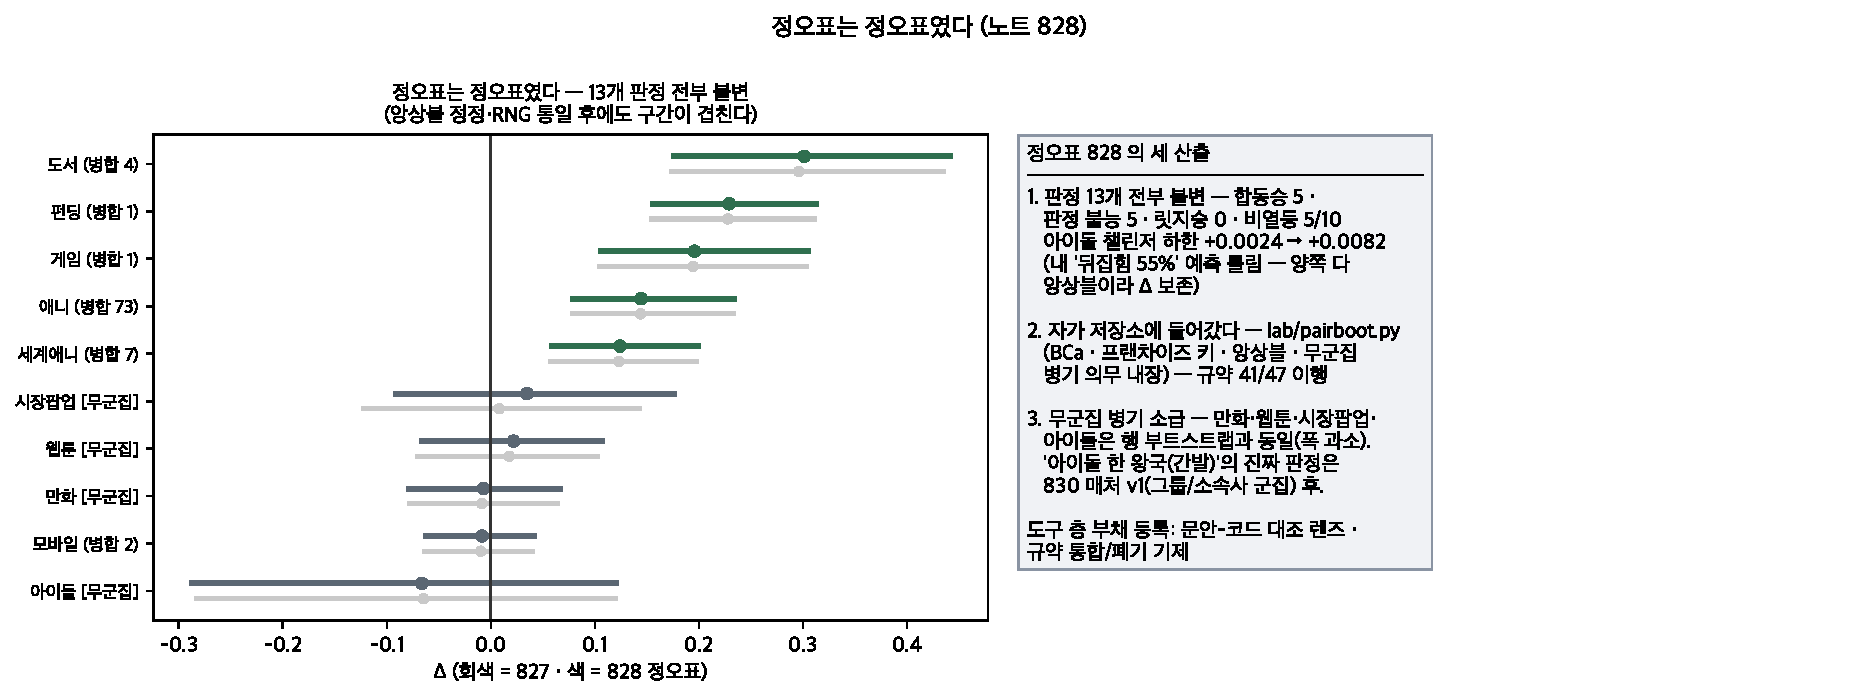
\includegraphics[width=0.97\textwidth]{figs/errata.pdf}
\caption{왼쪽: $827$(회색) 대 $828$(색) --- 구간이 겹친다. 오른쪽: 세 산출.}
\end{figure}

\section{판정보다 큰 것은 도구 층이다}

\claim{\textbf{규약 $47$ 의 자가 커밋된 코드가 됐다}(\texttt{lab/pairboot.py}
--- BCa · 프랜차이즈 키 v$0$ · rank\_ensemble · \textbf{무군집 병기 의무 내장}).
티처 \#$4$ 의 진단 --- \emph{``이 랩은 자기 문장은 세계 최고 수준으로
의심하는데 자기 도구는 아직 그만큼 의심하지 않는다''} --- 에 대한 첫 수리다.
무군집 병기를 $827$ 에 소급한다: 만화 · 웹툰 · 시장팝업 · 아이돌은 행
부트스트랩과 동일(폭 과소 방향)이었고, 특히 \textbf{`아이돌 한 왕국(간발)'의
진짜 판정은 $830$ 매처 v$1$}(아이돌 군집 열쇠 $=$ 그룹/소속사) \textbf{후로
미룬다.}}
{남은 도구 층 부채(등록): 적대 검증에 \textbf{사전등록 문안 대 코드 대조}
렌즈 추가(이번 구멍 ②가 통과한 자리) · $47$개로 자란 규약의 통합/폐기 기제.
다음 두 사이클(티처 \#$4$ 합의): $829$ 사람 게이트를 검토 게이트로(KOBIS 문
두드리기 --- 대장에 언급 $0$건 · 유튜브 목록 초안 자가 생성) · $830$
프랜차이즈 매처 v$1$. 판 $\rho$ $0.4689$ 그대로.}

\end{document}
